\chapter{Przetwarzanie danych zebranych z~odbiornika}

W ramach niniejszej pracy powstało oprogramowanie w \textit{Pythonie}, którego zadaniem jest
przekształcenie surowych danych ultradźwiękowych 
z odbiornika na informację o położeniu nadajnika w przestrzeni oraz jego orientacji.
Na oprogramowanie składają się biblioteka \textit{mp3d} zajmująca się
sterowaniem odbiornikiem, odbieraniem sygnałów ultradźwiękowych i ich analizą, program \textit{scan.py}
wizualizujący dane w postaci obrazu trójwymiarowego oraz program \textit{save-pattern.py},
który służy do wstępnej kalibracji urządzenia.

Najistotniejszą częścią oprogramowania jest biblioteka \textit{mp3d} podzielona na pięć modułów:
\begin{itemize}
 \item \textit{com.py} --  odpowiedzialny za komunikację z odbiornikiem,
 \item \textit{find\_pattern.py} --  wyznaczający odległości przez wyszukanie wzorca w odebranym sygnale,
 \item \textit{xyz.py} --  określający pozycję i orientację nadajnika oraz  weryfikujący, 
 czy zebrane dane odpowiadają modelowanej rzeczywistości,
 \item \textit{info.py} --  wyświetlający informację o sile odbieranego sygnału,
 \item \textit{ply.py} --  odpowiedzialny za eksportowanie danych do formatu \textit{.ply},
    (Polygon File Format) obsługiwanego przez większość programów do obróbki grafiki 3D.
\end{itemize}


\section{Komunikacja z odbiornikiem, moduł \textit{com.py}}

Za komunikację z odbiornikiem odpowiedzialny jest moduł \textit{com.py}.
Pracuje on w oddzielnym wątku, w którym cyklicznie wysyłane są żądania, by dany głośnik nadał sygnał,
a następnie odbierane są sygnały z trzech mikrofonów.
Ten proces odbywa się kolejno dla każdego z~czterech głośników nadajnika.
Zebrane w ten sposób dwanaście sygnałów po wstępnej filtracji przekazywane są dalej do \textit{find\_pattern.py}. Cały cykl powtarza 
się co \SI{350}{ms}. Rysunek \ref{fig:com_output_2m} przedstawia sygnał odebrany z jednego z mikrofonów.


\begin{figure}[h!]
    \centering
    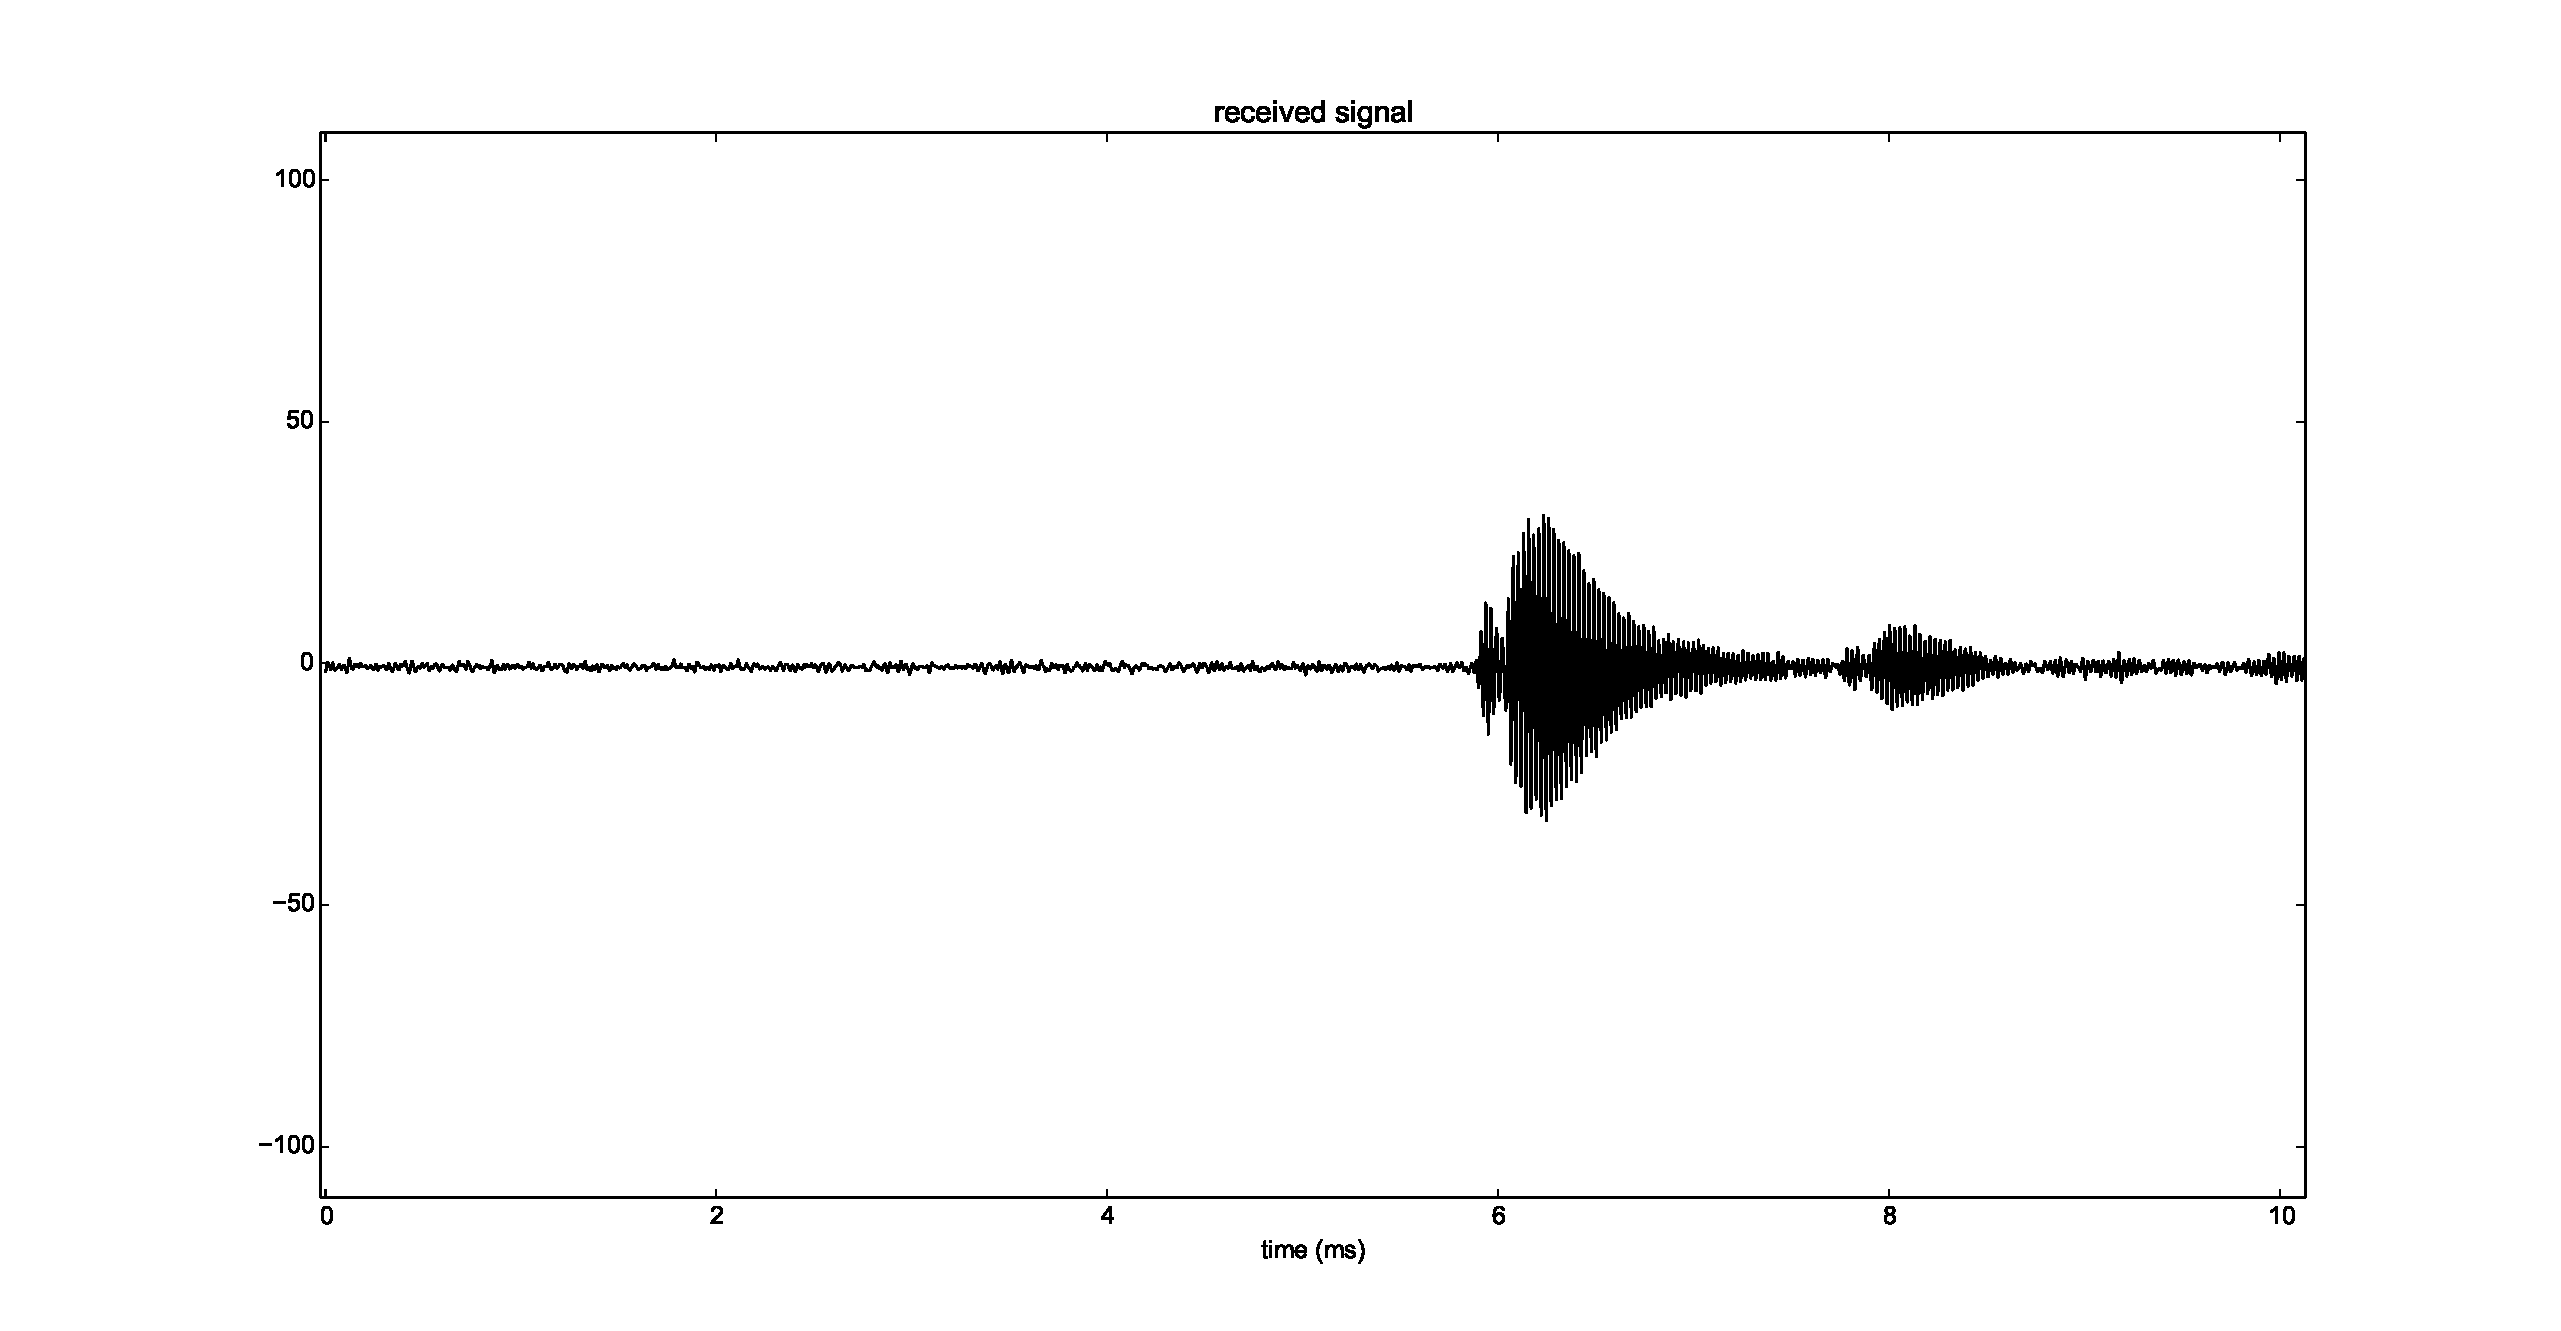
\includegraphics[width=1.13\textwidth, trim= 53mm 0mm 0mm 0mm,clip]{com_output_2m_1}
    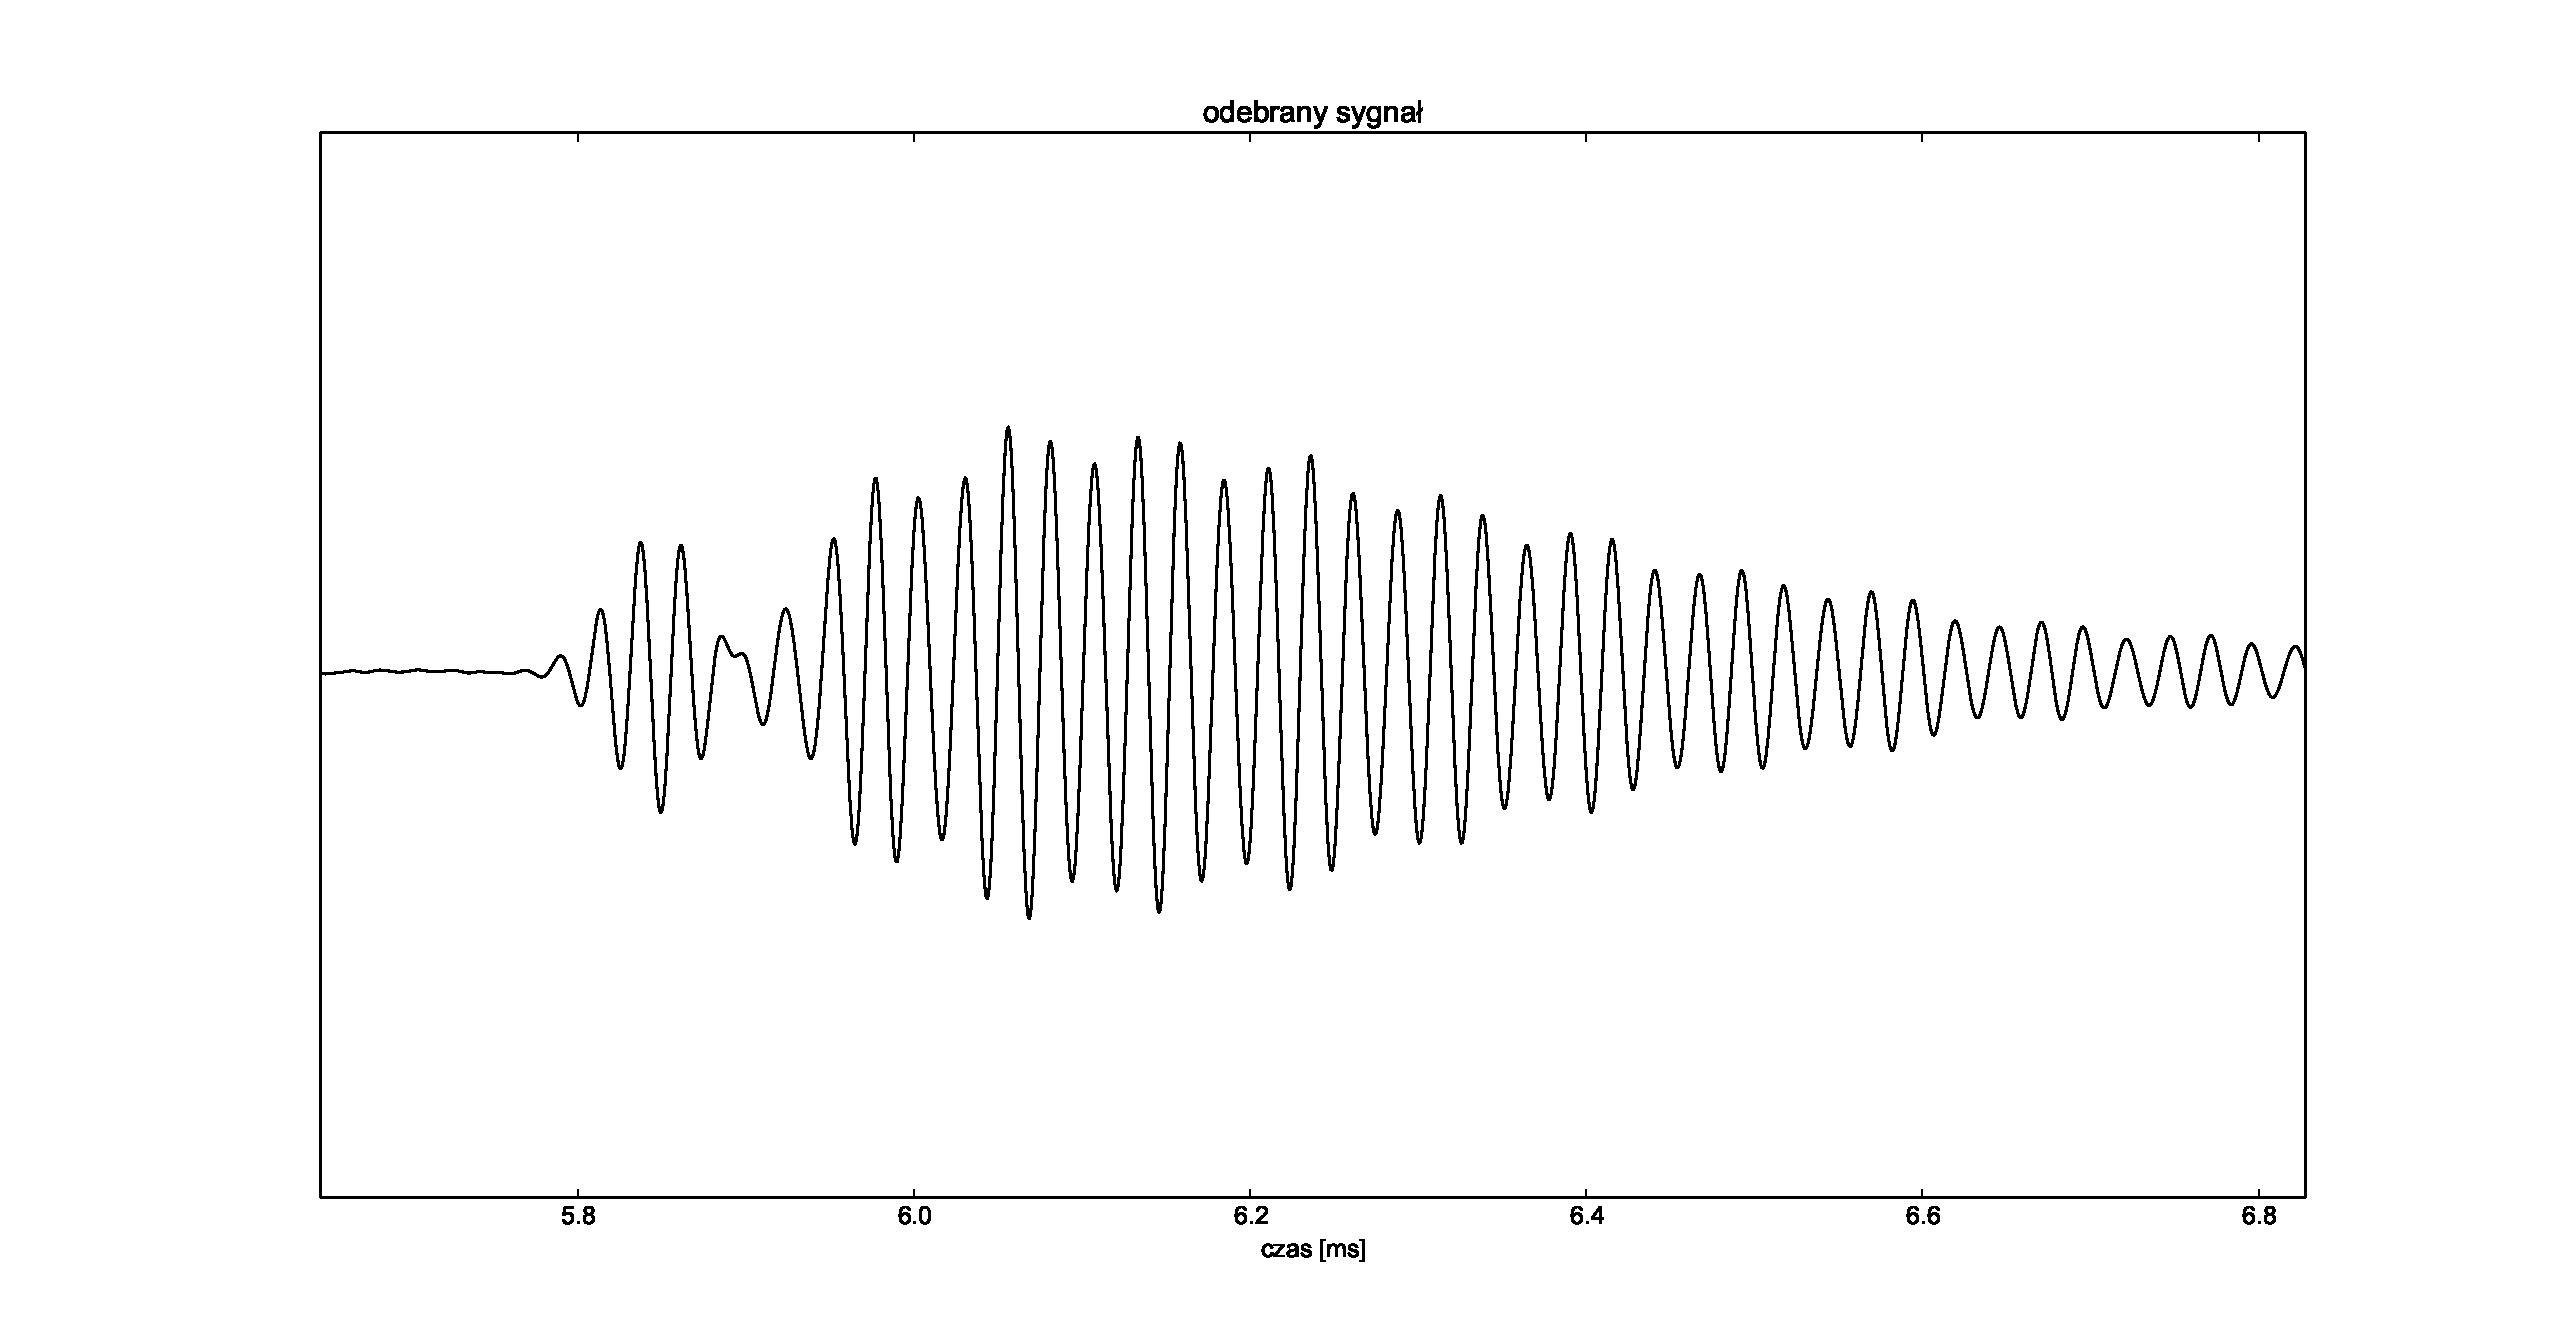
\includegraphics[width=1.13\textwidth, trim= 53mm 0mm 0mm 0mm,clip]{com_output_2m_2}
    \caption{Sygnał odebrany przez moduł \textit{com.py}. 
    Odległość między nadajnikiem a odbiornikiem wynosi 2 metry.
    Na górnym wykresie po prawej stronie widać również sygnały odbite od ścian}
    \label{fig:com_output_2m}
\end{figure}

\newpage
\section{Wyznaczanie odległości, moduł \textit{find\_pattern.py}}

Moduł \textit{find\_pattern.py} odpowiada za obliczenie odległości pomiędzy czterema głośnikami i~trzema mikrofonami.
Wyznaczana jest ona przez wyszukanie w każdym z 12 odebranych sygnałów  położenia \textit{wzorca}, który 
odpowiada czołu nadanego sygnału (rysunek \ref{fig:com_output_2m}).
\textit{Wzorzec} po raz pierwszy wprowadza się podczas kalibracji, a następnie ciągle aktualizuje 
(podmienia na sygnałem pasującym do \textit{wzorca}).

W celu wyszukania \textit{wzorca} wewnątrz sygnału korzysta się z  metody najmniejszego błędu średniokwadratowego:
Niech $w(t)$  dla $t = 0, ..., n-1$ będzie szukanym \textit{wzorcem}, a $f(x)$ dla $x = 0, ..., m-1$ odebranym sygnałem.
Wtedy możemy znaleźć takie $a$, że błąd średniokwadratowy $E(x)$ pomiędzy $w(t)$ i $a f(t+x)$ jest minimalny.
Możemy to zapisać w postaci
\[
  E(x) = \min_{a \in R} \{ \sum_{t=0}^{n-1}  (w(t) - a f(t+x))^2 \}.
\]
Po podniesieniu wyrażenia w nawiasie do kwadratu otrzymujemy
\[
  E(x) = \min_{a \in R} \{ \sum_{t=0}^{n-1}  (w^2(t) -2a w(t) f(t+x) + a^2 f^2(t+x)) \},
\]
\[
  E(x) = \min_{a \in R} \{ \sum_{t=0}^{n-1}  w^2(t) -2a \sum_{t=0}^{n-1}  w(t) f(t+x) + a^2 \sum_{t=0}^{n-1} f^2(t+x) \}.
\]
Aby wyliczyć $E(x)$, należy zminimalizować wyrażenie
\[
  y(a) = \sum_{t=0}^{n-1}  w^2(t) -2a \sum_{t=0}^{n-1}  w(t) f(t+x) + a^2 \sum_{t=0}^{n-1} f^2(t+x).
\]
Korzystając z faktu, że $y(a)$ jest funkcją kwadratową, możemy wyliczyć $a$ minimalizujące $y(a)$
\[
  a = \frac{ \sum\limits_{t=0}^{n-1}  w(t) f(t+x) }{ \sum\limits_{t=0}^{n-1} f^2(t+x) }.
\]
Ostatecznie dostajemy wzór na $E(x)$
\[
  E(x) = \sum_{t=0}^{n-1}  w^2(t)  - \frac {\left(\sum\limits_{t=0}^{n-1}  w(t) f(t+x) \right)^2 } { \sum\limits_{t=0}^{n-1} f^2(t+x)}.
\]

Zauważmy, że dzięki skalowaniu skalarem $a$  sygnału $f(x)$, a nie \textit{wzorca} $w(x)$,
otrzymane $E(x)$ nie zależy od siły odebranego sygnału. Ułatwia to porównanie błędów w dwóch różnych miejscach.
$E(x)$ zależy jednak od siły sygnału wzorcowego -- możemy się od niego  uniezależnić, wyznaczając
błąd względny $e(x)$
\[
  e(x) = \frac{E(x)}{\sum\limits_{t=0}^{n-1}  w^2(t)}.
\]
Po podstawieniu $E(x)$ dostajemy
\[
  e(x) = 1 - \frac {\left(\sum\limits_{t=0}^{n-1}  w(t) f(t+x) \right)^2 } { \sum\limits_{t=0}^{n-1} f^2(t+x) \sum\limits_{t=0}^{n-1}  w^2(t)}.
\]
 
 Funkcję $e(x)$  można interpretować następująco:
 im mniejszy błąd $e(x)$, tym większe prawdopodobieństwo, że szukany \textit{wzorzec} $w$ znajduje się na pozycji $x$ w 
 odebranym sygnale $f$. 

 Wynikiem obliczeń modułu \textit{find\_pattern.py} jest cała funkcja $e(x)$, na podstawie której moduł \textit{xyz.py}
 wyznacza pozycję i orientację nadajnika, uwzględniając przy tym 
 jego kształt (nadmiarowość danych), a także prawdopodobieństwo, że znaleziony \textit{wzorzec} znajduje się w określonej pozycji.
 Rysunek \ref{fig:blad_korel} przedstawia wynik przetwarzania sygnału przez moduł \textit{find\_pattern.py}.

\begin{figure}[h!]
    \centering
    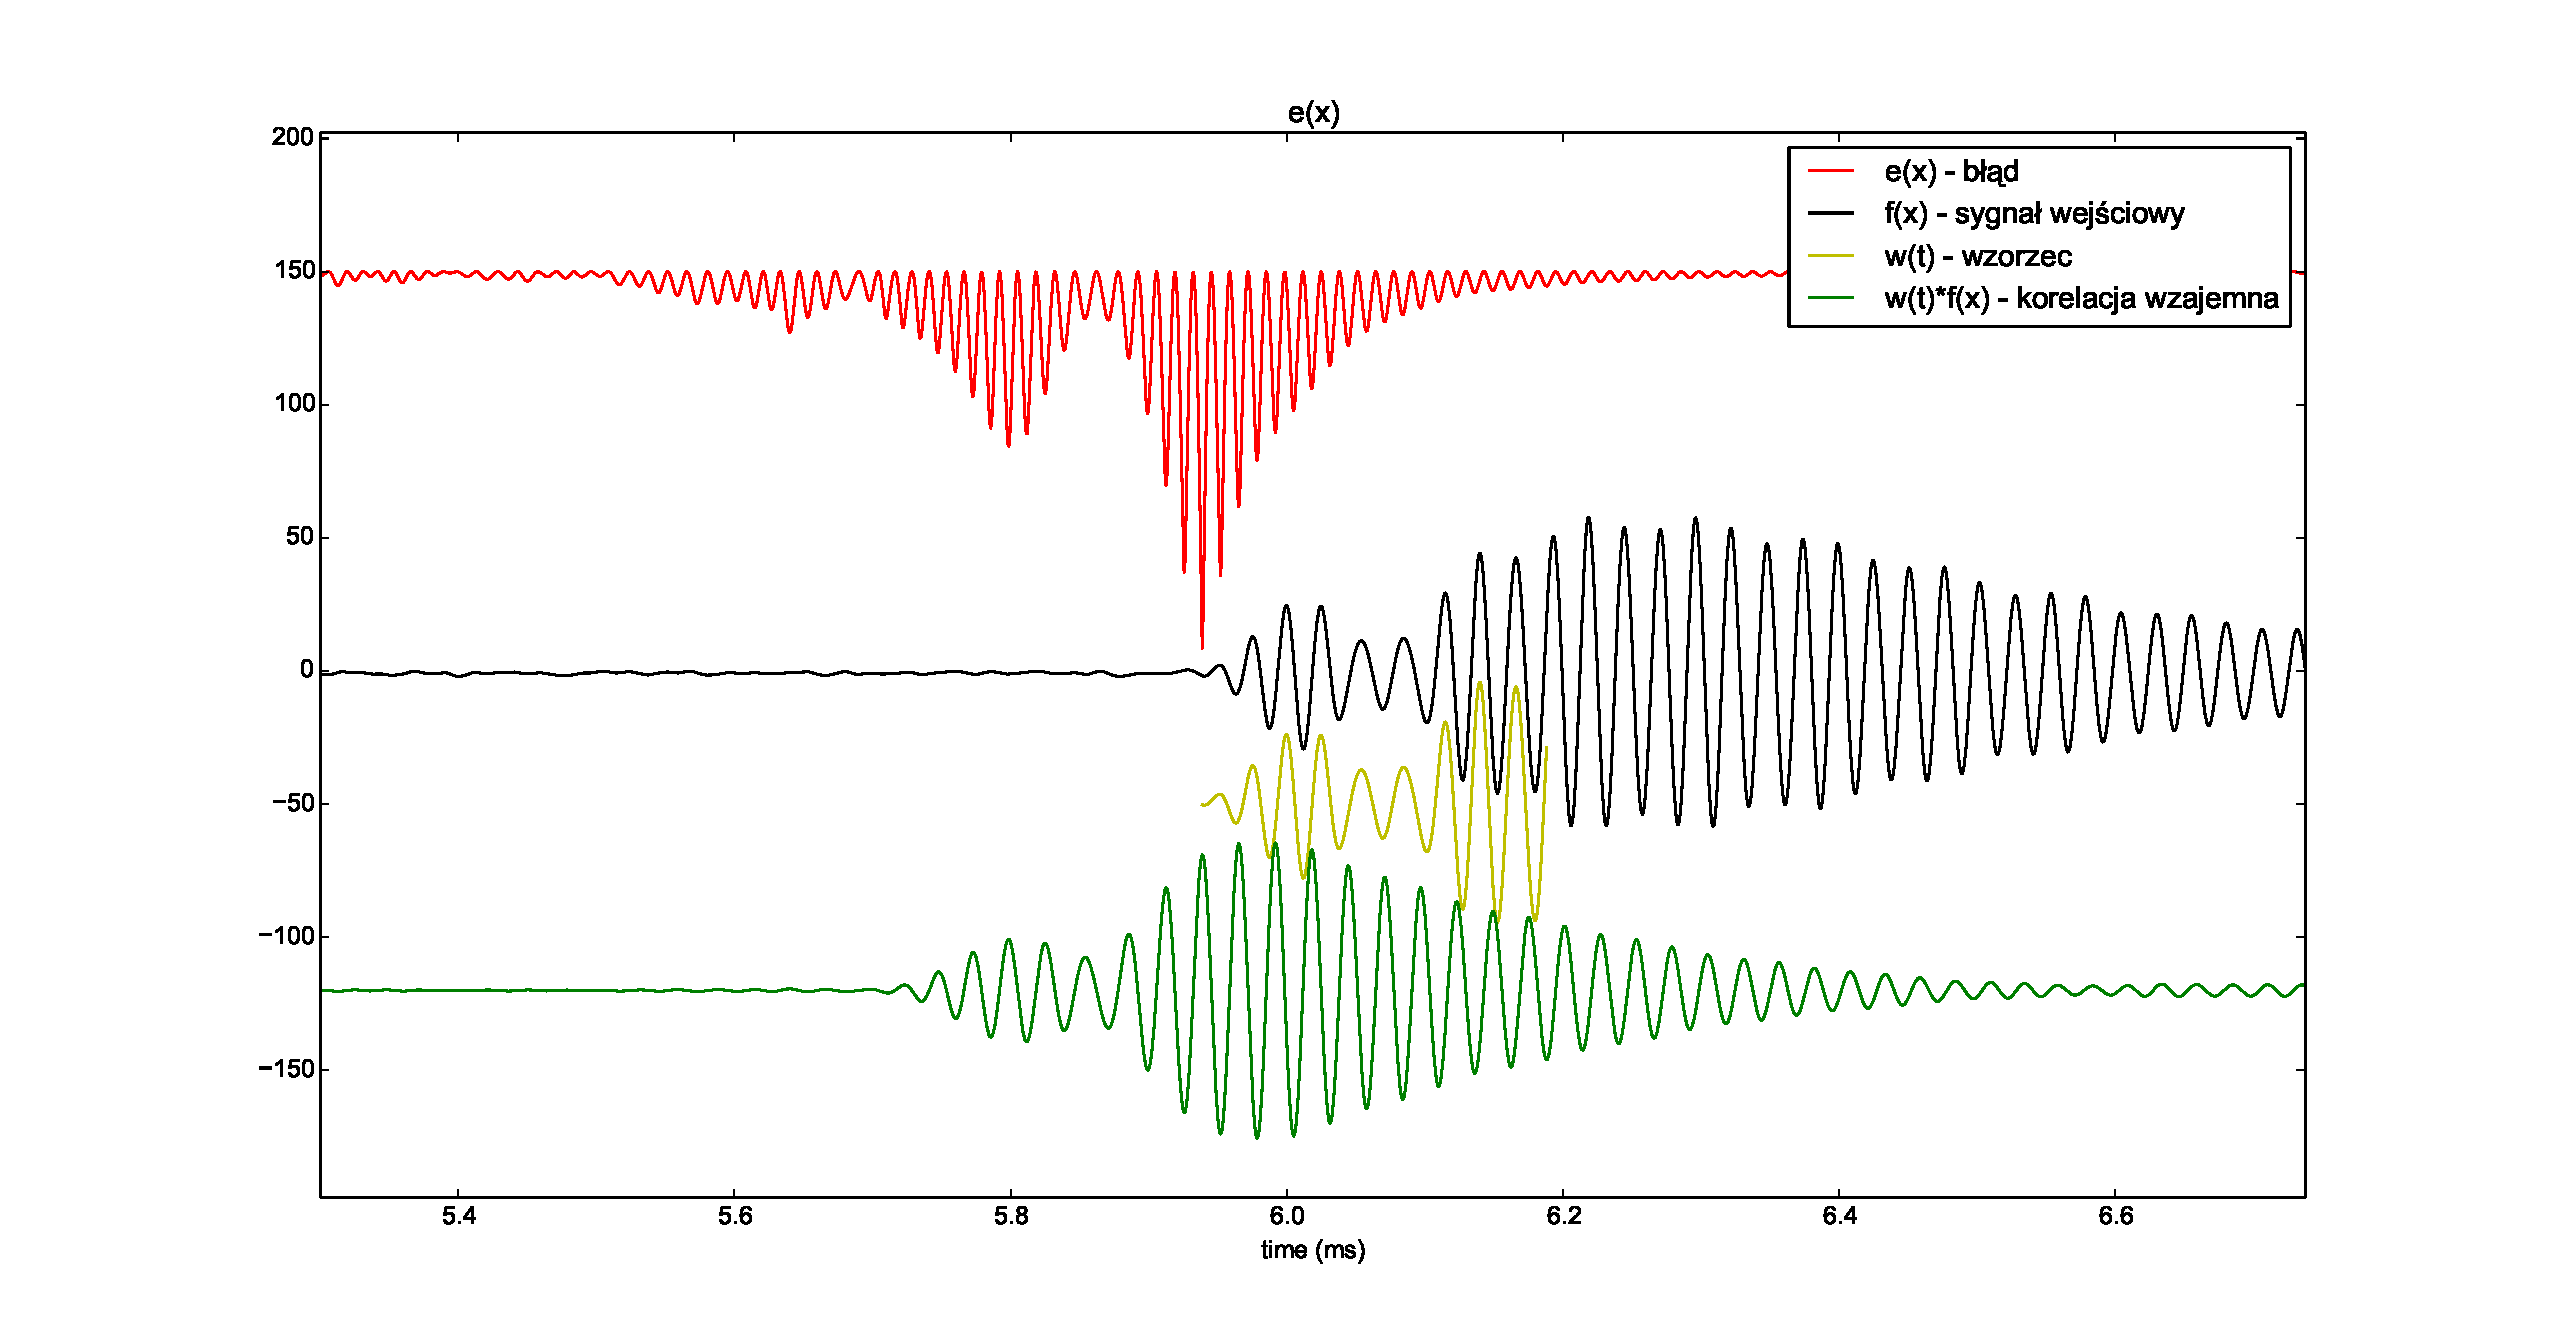
\includegraphics[width=1.13\textwidth, trim= 53mm 0mm 0mm 0mm,clip]{blad_korel}
    \caption{Sygnał przetworzony przez moduł \textit{find\_pattern.py}}
    \label{fig:blad_korel}
\end{figure}
 
 
 Analiza złożoności obliczeniowej: wyliczenie zarówno $ \sum\limits_{t=0}^{n-1}  w^2(t) $,
jak i $\sum\limits_{t=0}^{n-1} f^2(t+x)$ wymaga jedynie liniowej liczby operacji, a 
 $\sum\limits_{t=0}^{n-1}  w(t) f(t+x) $ jest korelacją wzajemną funkcji $w(t)$ i $f(x)$, którą
 można wyliczyć w czasie $m \log(m)$, korzystając z szybkiej transformacji Fouriera \cite{bib:FFT_correlation},
 gdzie $m = \max \{|w|, |f| \}$. Wyliczenie całej funkcji $e(x)$ wymaga zatem jedynie $m \log(m)$ operacji.

 
 Kolejnym zadaniem modułu \textit{find\_pattern.py} jest uaktualnianie \textit{wzorca}.
 Wraz ze zmianą kąta nachylenia nadajnika względem odbiornika zmienia się kształt odbieranego sygnału,
 dlatego jeśli badany sygnał zawiera szukany \textit{wzorzec} oraz spełnione są następujące warunki:
 \begin{itemize}
  \item moc sygnału pasującego do \textit{wzorca} jest wystarczająco duża,
  \item błąd względny pomiędzy sygnałem a \textit{wzorcem} jest mały,
  \item moduł \textit{xyz.py} rozpozna otrzymane pozycje jako pasuje do modelowanej rzeczywistości
 \end{itemize}
to moduł uaktualni \textit{wzorzec}.
 
 
\section{Wyznaczanie pozycji oraz orientacji przestrzennej, moduł \textit{xyz.py}}

Na ostatnim etapem obliczeń wyznaczane są współrzędne kartezjańskie czterech głośników umieszczonych na nadajniku.
Zajmuje się tym moduł \textit{xyz.py}, który dodatkowo zawiera prosty model rzeczywistości
wyłapujący niepoprawne dane o położeniu głośników.
Niepoprawne dane powstają, gdy część głośników traci widoczność z mikrofonami, np. gdy zostaną przysłonięte.
W ramach modelowanej rzeczywistości określa się:
\begin{itemize}
  \item prędkość, z jaką porusza się każdy z głośników,
  \item kształt nadajnika -- położenie głośników względem siebie w przestrzeni.
\end{itemize}
Jeśli któreś z wyliczeń odbiega od ustalonej normy, to dany pomiar uznawany jest za błędny.


Współrzędne głośników wyznacza się na podstawie dwunastu funkcji $e_{ij}(x)$ dla $i=1, ..., 4$ oraz $j=1, ..., 3$,
w których zawarta jest informacja o odległości pomiędzy głośnikiem $i$ oraz mikrofonem $j$.
Dla każdej funkcji $e_{ij}(x)$ wyszukiwane są pozycje minimów lokalnych, 
z których następnie wybierane jest $t$ pozycji $x^{ij}_1, ..., x^{ij}_t$
o najmniejszych wartościach, gdzie $t$ jest stałą wewnętrzną modułu \textit{xyz.py}.
Pozycje $x^{ij}_k$ dla $k=1, ..., t$  można interpretować jako najbardziej prawdopodobne odległości pomiędzy głośnikiem, a mikrofonem.

Do wyliczenia położenia głośników wykorzystywane są wszystkie możliwe kombinacje wyznaczonych odległości.
Zauważmy, że jest ich $12^t$. Każda z tych kombinacji 
sprawdza się czy pasuje do modelowanej rzeczywistości. Z tych, które są akceptowalne, wybierana jest 
kombinacja o najmniejszym sumarycznym błędzie średniokwadratowym, czyli najbardziej prawdopodobna.

Ostatecznym wynikiem pracy modułu \textit{xyz.py} są wartości $x^{ij}$, czyli najbardziej prawdopodobne odległości
pomiędzy  $i$-tym głośnikiem (gdzie $i=1,...,4$), a $j$-tym mikrofonem, na podstawie których 
wyznacza się  pozycję oraz orientację nadajnika.

Wartości $x^{ij}$ przekazywane są również z powrotem do modułu \textit{find\_pattern.py} w celu aktualizacji \textit{wzorców}.


\section{Kalibracja}

Przed każdym uruchomieniem urządzenie wymagana kalibracji,
która sprowadza się do ustawienia nadajnika w odległości 2 metrów od odbiornika,
uruchomienia programu \textit{save-pattern.py} oraz zaznaczenia  12 obszarów  będącym czołem odebranego sygnału.
Obszary te wykorzystane zostaną jako \textit{wzorce} podczas mierzenia odległości.
Program wyliczy także aktualną prędkość dźwięku, uwzględniając odległość nadajnika od odbiornika.

Rysunek \ref{fig:kalibracja_12x} przedstawia 12 sygnałów wraz z zaznaczonymi wzorcami.


 \begin{figure}[h!]
    \centering
    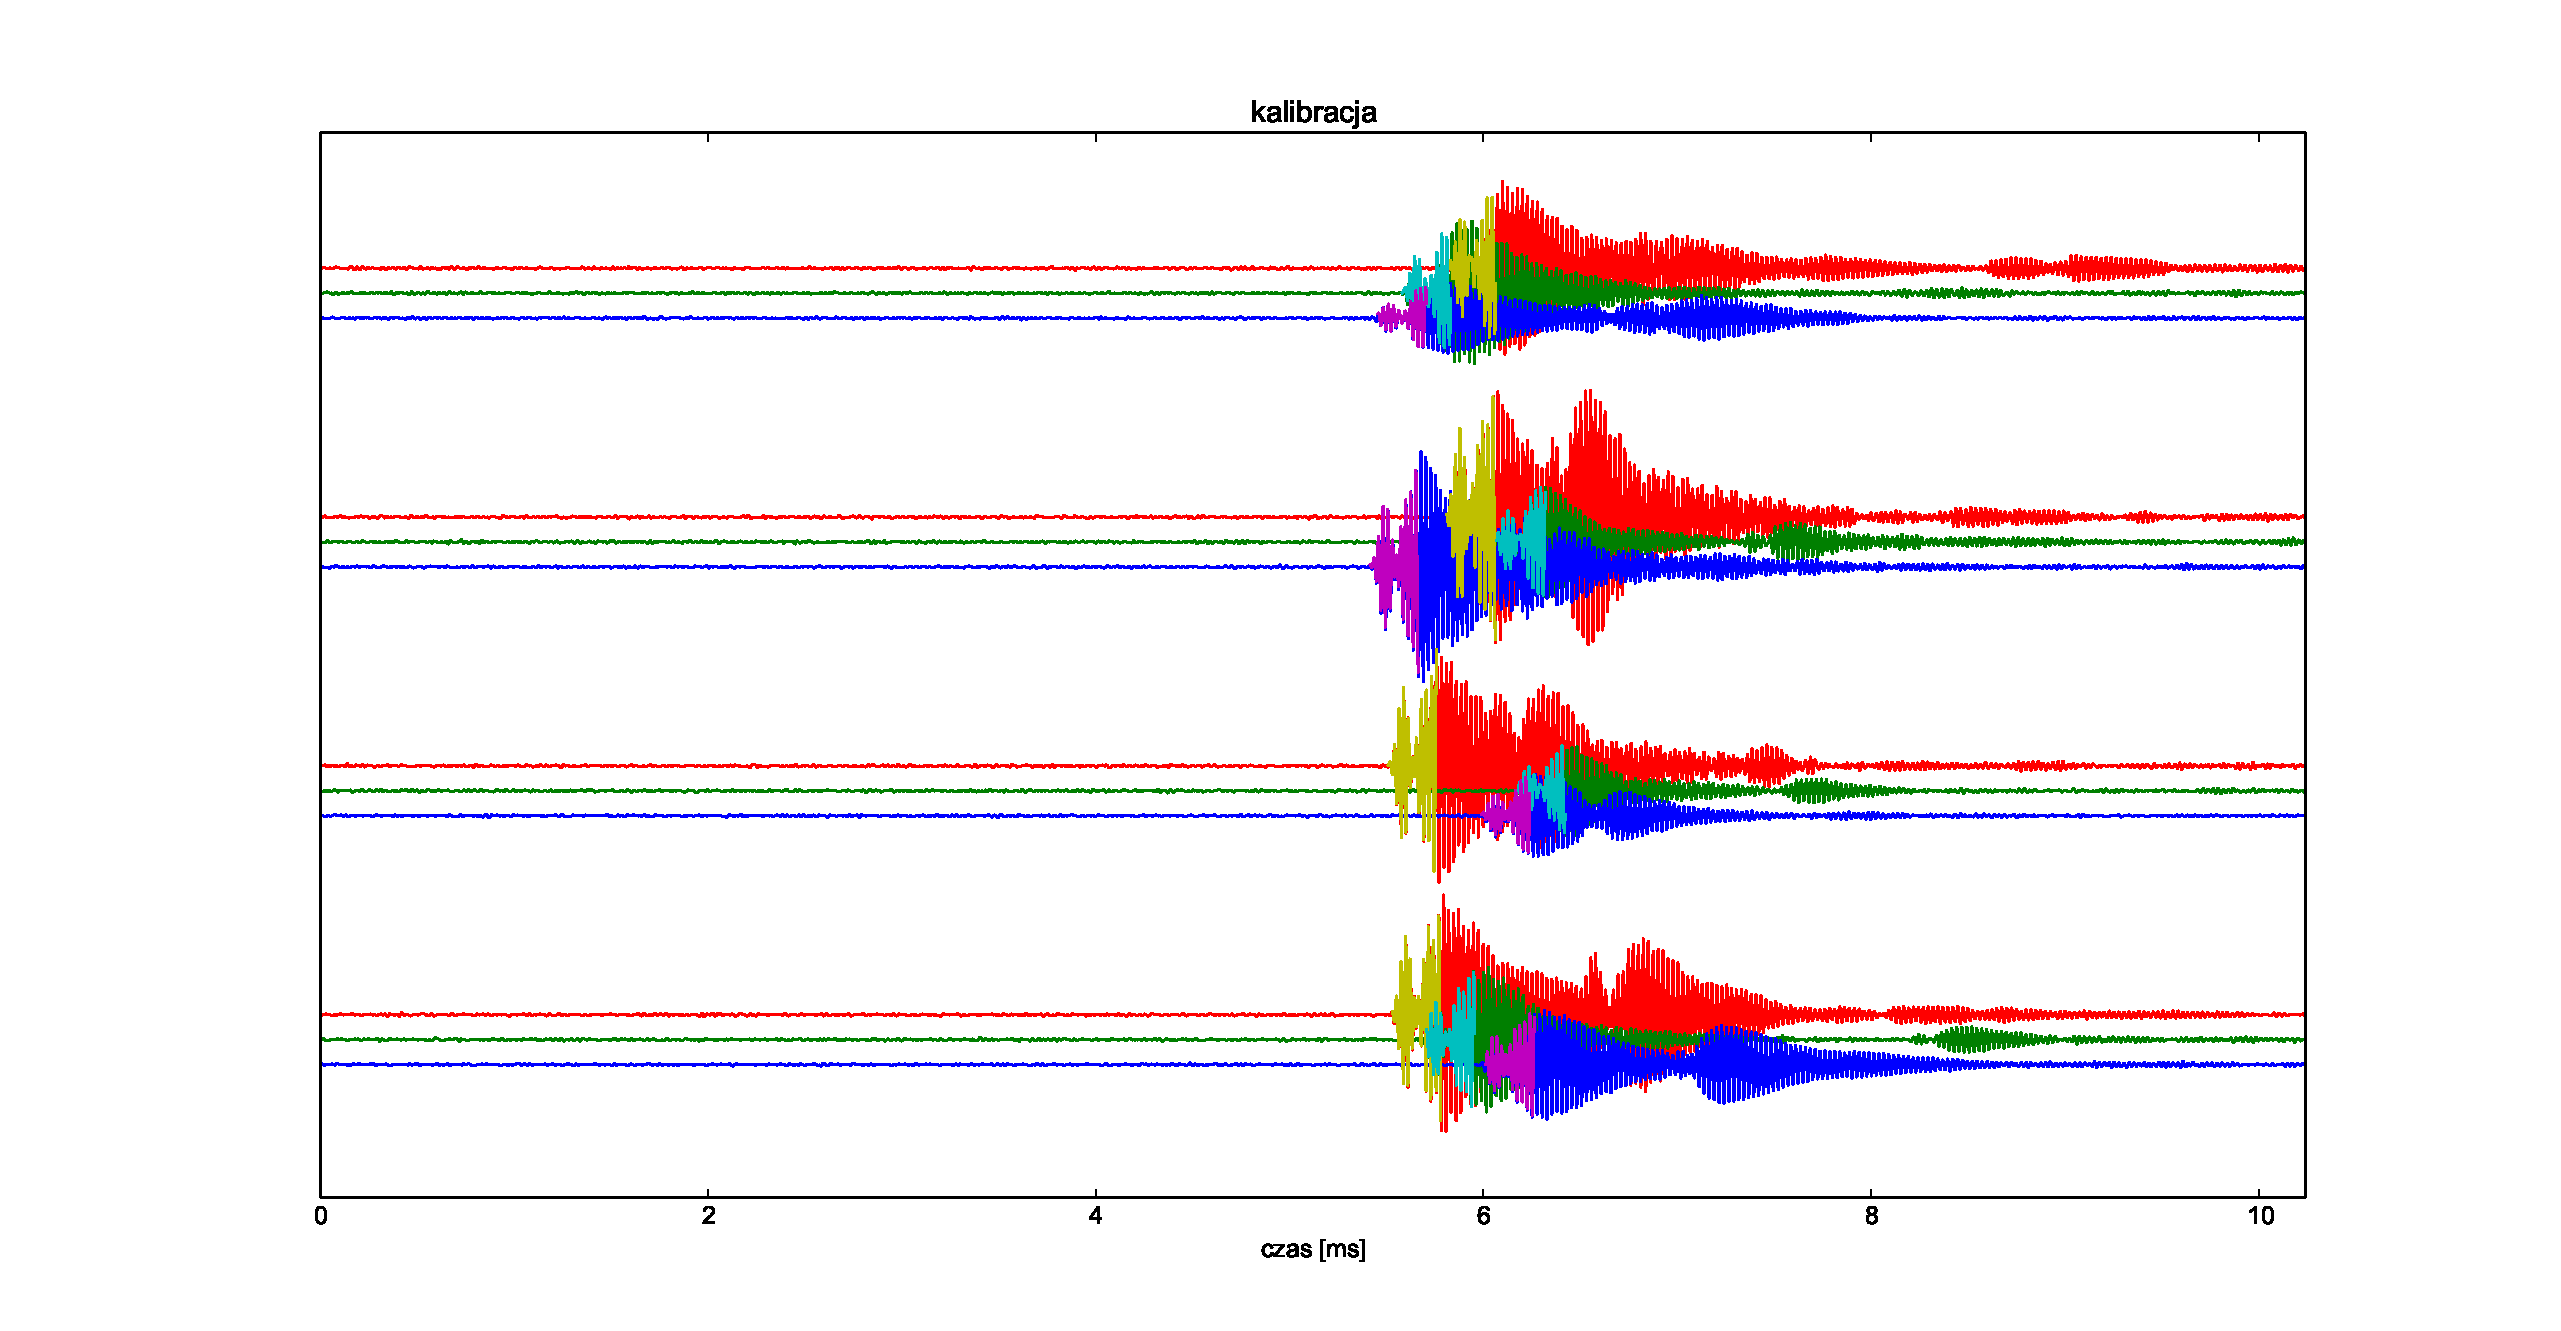
\includegraphics[width=1.12\textwidth, trim= 46mm 0mm 0mm 0mm,clip]{kalibracja_12x}
    \caption{Kalibracja, 12 sygnałów z zaznaczonymi \textit{wzorcami}}
    \label{fig:kalibracja_12x}
\end{figure}

\newpage

\section{Obsługa programu \textit{scan.py}}

Do obsługi prototypu służy program \textit{scan.py}. Po jego uruchomieniu 
na monitorze wyświetlają się trzy okna: 
\begin{itemize}
 \item widok 3D prezentujący położenie nadajnika w przestrzeni -- w oknie widoczne są  
 cztery punkty reprezentujące głośniki nadajnika oraz trzy prostopadłe względem siebie wektory określające 
jego orientację i położenie (rysunek \ref{fig:widok3d}),
 \item widok 2D, również przestawiające położenie nadajnika w przestrzeni --
 są to nałożone na siebie rzuty na płaszczyzny XY i XZ
 (rysunek \ref{fig:widok2d}),
 \item diagram informujący o mocy całego odebranego sygnału, mocy \textit{wzorca}, mocy sygnału pasującego do \textit{wzorca} 
 oraz błędzie pomiędzy \textit{wzorcem} a odebranym sygnałem (rysunek \ref{fig:power}).
\end{itemize}

Wszelkie zmiany położenia nadajnika automatycznie odświeżają wszystkie widoki. 
Podczas uruchamiania programu aktualne położenie nadajnika przyjmowane 
jest jako początek układu współrzędnych.
Jeśli któryś z głośników straci widoczność z mikrofonami, obraz przestaje się odświeżać, a informacja, dlaczego tak
się dzieje, widoczna jest w oknie przedstawiającym moc sygnału.


\rysunek{3d}{Widok 3D}{\label{fig:widok3d}}
\rysunek{2d}{Widok 2D}{\label{fig:widok2d}}
\rysunek{power}{Diagram informujący o mocy całego odebranego sygnału, mocy \textit{wzorca}, mocy sygnału pasującego do \textit{wzorca} 
 oraz błędzie pomiędzy \textit{wzorcem} a odebranym sygnałem}{\label{fig:power}}

